
\subsection{2項ヒープ}
\frame{
  \frametitle{2項ヒープ}
  \begin{block}{Binomial Heap}
    全順序集合$P(C,\leq)$について,$C$上からなる要素の二項ヒープは\\
    以下の操作が実行できる
    \itemize{
    \item top : $O(\log N)$でヒープの最大値を求める
    \item \alert{merge : $O(\log (N+M))$で2つのヒープを併合する}
    \item push : $O(\log N)$で$C$の要素$x$を追加する
    \item pop : $O(\log N)$でヒープの最大値をもつ要素を削除する
    \item delete : $O(\log N)$で与えられたポインタの先の要素を消去する
    \item replace : $O(\log N)$で$C$の要素$x$ヒープの最大値をもつ要素を置き換える\\ 
    }
    ヒープ条件を満たす2項木の集合
  \end{block}
}

\frame{
  \frametitle{2項木}
  \begin{block}{Binomial Tree}
    $B_0$は1個の頂点から構成される.
    $B_k$は2つの$B_{k-1}$から構成され,
    片方の根がもう一方の根の最も左の子になるように連結される.
  \end{block}
  \begin{exampleblock}{例}
    \center{
      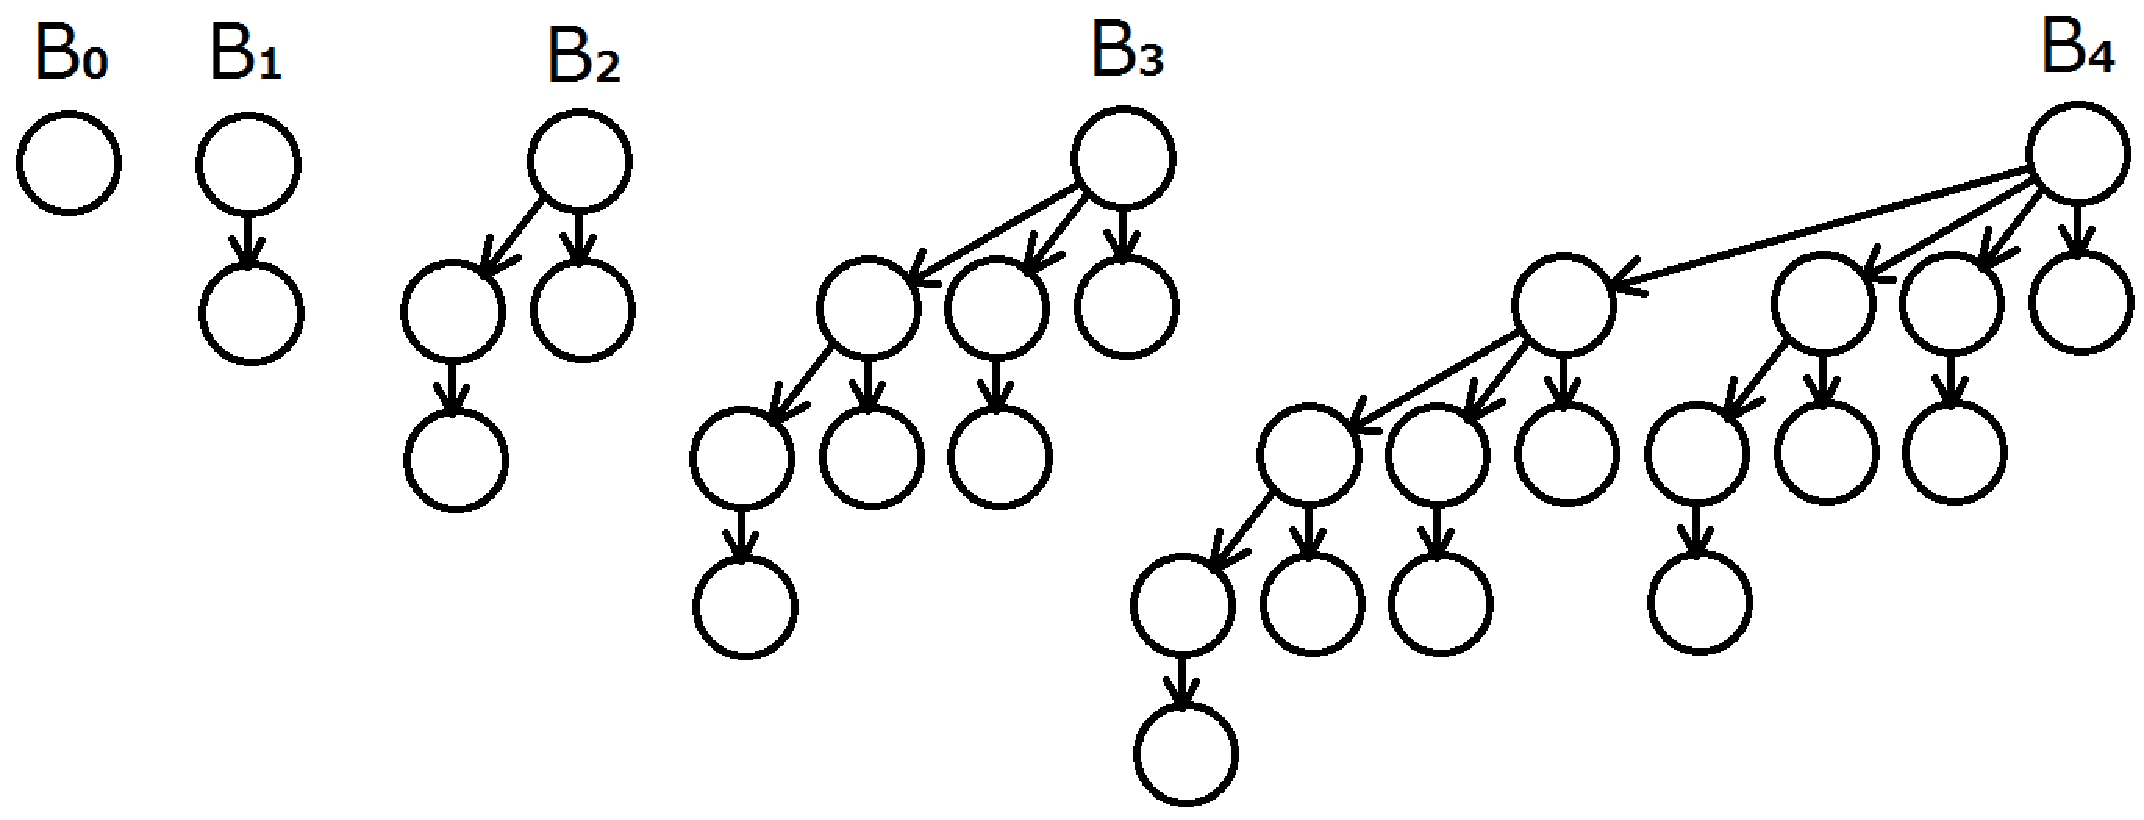
\includegraphics[width=10cm]{image/binomial01.pdf}
    }
  \end{exampleblock}
}

\frame{
  \frametitle{2項木}
  \begin{block}{Binomial Tree}
    各接点は,親を指すポインタ,最も左の子を指すポインタ,\\
    直接右の兄弟を指すポインタを含んでいる.
  \end{block}
  \begin{exampleblock}{例}
    \center{
      \includegraphics<1>[width=10cm]{image/binomial02.pdf}
      \includegraphics<2>[width=3.4cm]{image/binomial03.pdf}
    }
  \end{exampleblock}
}

\frame{
  \begin{block}{Binomial Heap}
    2項ヒープは2項木を小さい順に左から並べた集合として\\
    表現される.
  \end{block}
  \begin{exampleblock}{例}
    \center{
      \includegraphics<1>[width=7cm]{image/binomial04.pdf}
      \includegraphics<2>[width=7cm]{image/binomial05.pdf}
    }
  \end{exampleblock}
}

\frame{
  \frametitle{top}
  \begin{block}{top$(H)$}
    1.  $y \leftarrow$ nil\\
    2.  $x \leftarrow head(H)$\\
    3.  $max \leftarrow -\infty$\\
    4.  {\bf While} $x \neq$ nil {\bf do}\\
    5. ~~ {\bf If} $key[x] > max$\\
    6. ~~~~~ {\bf Then} $max \leftarrow key[x]$\\
    7. ~~~~~~~~~~~~~~ $y \leftarrow x$\\
    8. ~~ $x \leftarrow sibling[x]$\\
    9.  return $y$
  \end{block}
}

\frame{
  \frametitle{top}
  \begin{block}{top}
    各2項木の根の中で最大値を探す.$O(\log N)$
  \end{block}
  \begin{exampleblock}{例}
    \center{
      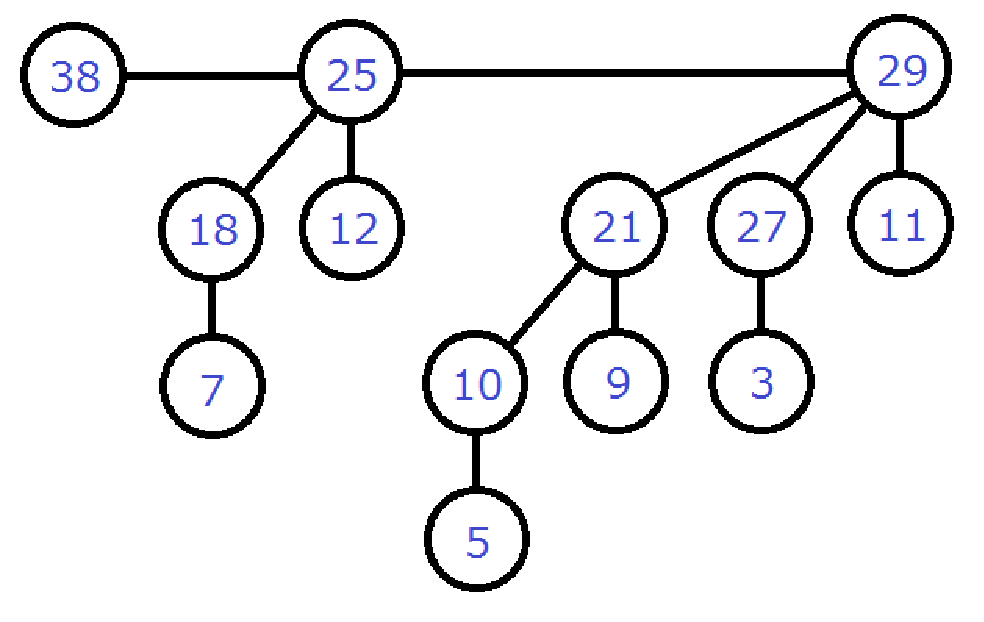
\includegraphics[width=7cm]{image/binomial05.pdf}
    }
  \end{exampleblock}
}

\frame{
  \frametitle{merge}
  \begin{block}{merge$(H_1, H_2)$}
    1.  各2項木を小さい順にmix\\
    2.  $x \leftarrow head(H)$\\
    3.  {\bf While} $sibling(x) \neq$ nil {\bf do}\\
    4. ~~ {\bf If} $deg[x] = deg[sibling(x)] \neq deg[sibling(sibling(x))]$\\
    5. ~~~~~ {\bf Then} $x$と$sibling(x)$の2つの二項木をmerge\\
    6. ~~~~~ {\bf Else} $x \leftarrow sibling(x)$
  \end{block}
  元の$H_1, H_2$は破壊される
}

\frame{
  \only<1-6>{
    \frametitle{merge}
    \begin{block}{merge}
      \only<1>{2つの2項ヒープを併合する}
      \only<2>{2項木を小さい順に併合する}
      \only<3-6>{小さい順に同じサイズのヒープがあれば併合する}
    \end{block}
  }
  \only<7>{
    \frametitle{push}
    \begin{block}{push}
      1要素のみからなる二項ヒープをmergeする
    \end{block}
  }
  \begin{exampleblock}{例}
    \center{
      \includegraphics<1>[width=10cm]{image/binomial06.pdf}
      \includegraphics<2>[width=10cm]{image/binomial07.pdf}
      \includegraphics<3>[width=10cm]{image/binomial08.pdf}
      \includegraphics<4>[width=10cm]{image/binomial09.pdf}
      \includegraphics<5>[width=10cm]{image/binomial10.pdf}
      \includegraphics<6->[width=9cm]{image/binomial11.pdf}
    }
  \end{exampleblock}
}

\frame{
  \frametitle{pop}
  \begin{block}{pop$(H)$}
    1.  $x \leftarrow top(H)$\\
    2.  $H$から接点$x$以下の2項木を除く\\
    3.  $x$の子の$sibling$のリストを逆順に繋ぎ,\\
    ~~~ 出来た2項ヒープを$H'$とする\\
    4.  merge $(H,H')$
  \end{block}
  元の$H_1, H_2$は破壊される
}

\frame{
  \frametitle{pop}
  \begin{block}{pop}
    \only<1>{最大値の要素を調べる}
    \only<2-3>{最大値を消す}
    \only<4-5>{最大値の要素の子だったものを小さい順に併合する}
    \only<6>{残った2つの二項ヒープをmergeする}
  \end{block}
  \begin{exampleblock}{例}
    \center{
      \includegraphics<1>[width=7cm]{image/binomial12.pdf}
      \includegraphics<2>[width=7cm]{image/binomial13.pdf}
      \includegraphics<3>[width=7cm]{image/binomial14.pdf}
      \includegraphics<4>[width=7cm]{image/binomial15.pdf}
      \includegraphics<5-6>[width=7cm]{image/binomial16.pdf}
    }
  \end{exampleblock}
}

\frame{
  \frametitle{delete}
  \begin{block}{delete$(H, x)$}
    1.  $x \leftarrow \infty$\\
    2.  {\bf While} $parent(x) \neq$ nil {\bf do}\\
    3. ~~ $key[x] \leftrightarrow key[parent(x)]$\\
    4. ~~ $x \leftarrow parent(x)$
    5.  $pop(H)$
  \end{block}
  元の$H_1, H_2$は破壊される
}

\frame{
  \frametitle{delete}
  \begin{block}{delete}
    \only<1>{値を$-\infty$に置き換える}
    \only<2>{ヒープ条件を満たすよう調整する}
    \only<3>{pop}
  \end{block}
  \begin{exampleblock}{例}
    \center{
      \includegraphics<1>[width=7cm]{image/binomial17.pdf}
      \includegraphics<2>[width=7cm]{image/binomial18.pdf}
      \includegraphics<3>[width=7cm]{image/binomial19.pdf}
    }
  \end{exampleblock}
}

\frame{
  \frametitle{replace}
  \begin{block}{replace$(H, k)$}
    1.  pop $(H)$\\
    2.  push $(H, k)$
  \end{block}
}
